\documentclass{standalone}
\usepackage{tikz}
\usetikzlibrary{patterns, positioning}
\usepackage[sfdefault]{ClearSans} %% option 'sfdefault' activates Clear Sans as the default text font
\usepackage[T1]{fontenc}

\begin{document}
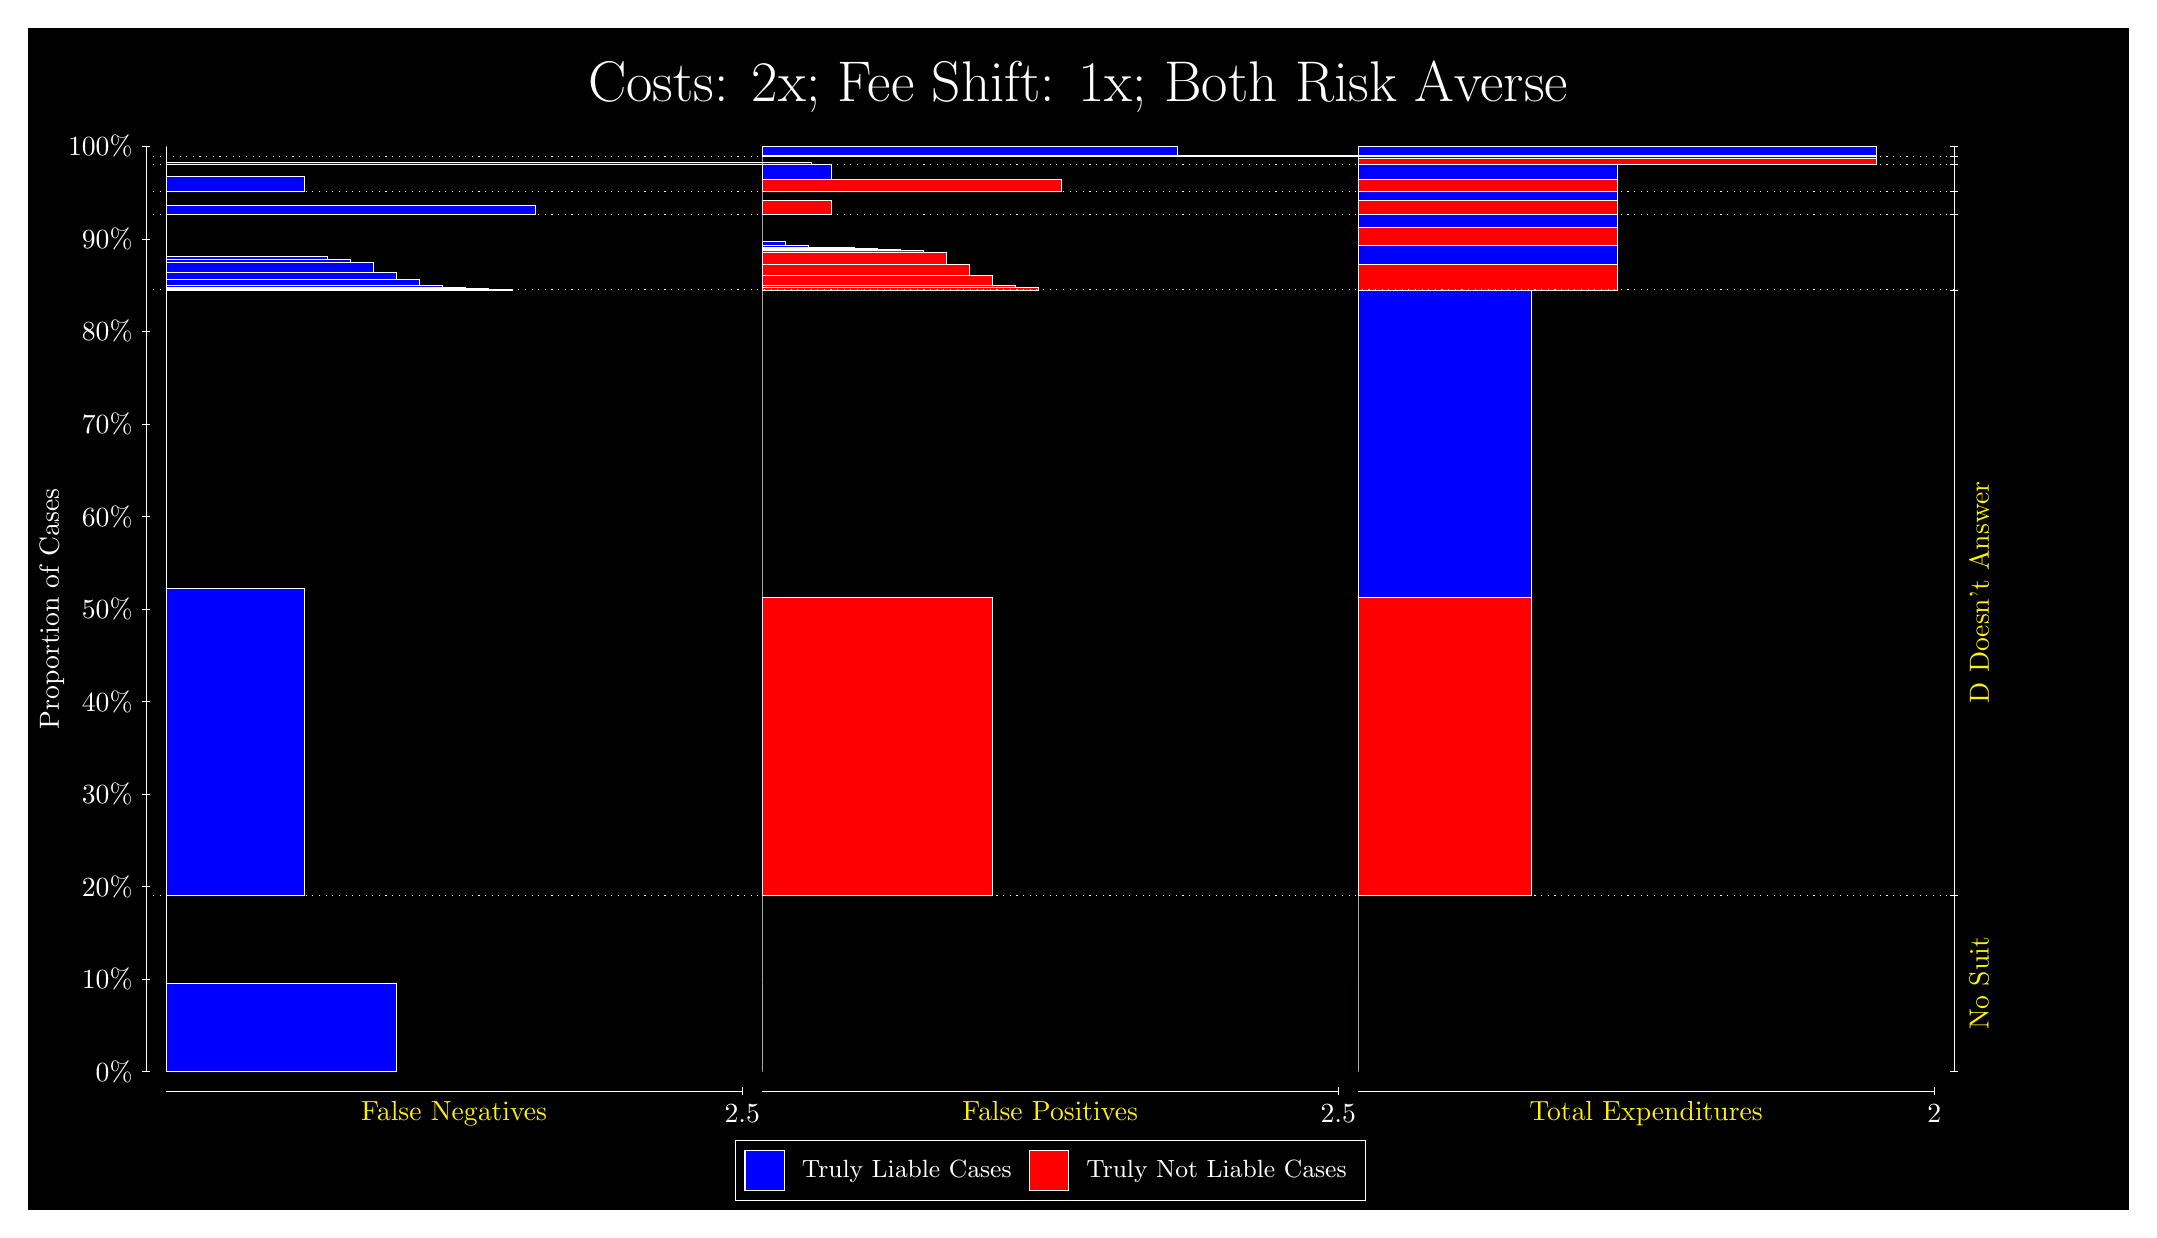
\begin{tikzpicture}
\draw[fill=black] (0,0) rectangle (26.667,15);
\draw[text=white] (0,13.5) rectangle (26.667,15) node[midway] {\huge Costs: 2x; Fee Shift: 1x; Both Risk Averse};
\draw[white, very thin] (1.5,1.75) -- (1.5,13.5);
\node[rotate=90, text=white, anchor=center] at (0.3, 7.625) {Proportion of Cases};
\draw[white, very thin] (1.45,1.75) -- (1.55,1.75);
\node[text=white, anchor=east] at (1.45, 1.75) {0\%};
\draw[white, very thin] (1.45,2.925) -- (1.55,2.925);
\node[text=white, anchor=east] at (1.45, 2.925) {10\%};
\draw[white, very thin] (1.45,4.1) -- (1.55,4.1);
\node[text=white, anchor=east] at (1.45, 4.1) {20\%};
\draw[white, very thin] (1.45,5.275) -- (1.55,5.275);
\node[text=white, anchor=east] at (1.45, 5.275) {30\%};
\draw[white, very thin] (1.45,6.45) -- (1.55,6.45);
\node[text=white, anchor=east] at (1.45, 6.45) {40\%};
\draw[white, very thin] (1.45,7.625) -- (1.55,7.625);
\node[text=white, anchor=east] at (1.45, 7.625) {50\%};
\draw[white, very thin] (1.45,8.8) -- (1.55,8.8);
\node[text=white, anchor=east] at (1.45, 8.8) {60\%};
\draw[white, very thin] (1.45,9.975) -- (1.55,9.975);
\node[text=white, anchor=east] at (1.45, 9.975) {70\%};
\draw[white, very thin] (1.45,11.15) -- (1.55,11.15);
\node[text=white, anchor=east] at (1.45, 11.15) {80\%};
\draw[white, very thin] (1.45,12.325) -- (1.55,12.325);
\node[text=white, anchor=east] at (1.45, 12.325) {90\%};
\draw[white, very thin] (1.45,13.5) -- (1.55,13.5);
\node[text=white, anchor=east] at (1.45, 13.5) {100\%};

\draw[white, very thin] (24.457,1.75) -- (24.457,13.5);
\draw[white, very thin] (24.407,1.75) -- (24.507,1.75);
\node[anchor=west] at (24.407, 1.75) {};
\draw[white, very thin] (24.407,3.9909) -- (24.507,3.9909);
\node[anchor=west] at (24.407, 3.9909) {};
\draw[white, very thin] (24.407,11.678) -- (24.507,11.678);
\node[anchor=west] at (24.407, 11.678) {};
\draw[white, very thin] (24.407,12.636) -- (24.507,12.636);
\node[anchor=west] at (24.407, 12.636) {};
\draw[white, very thin] (24.407,12.924) -- (24.507,12.924);
\node[anchor=west] at (24.407, 12.924) {};
\draw[white, very thin] (24.407,13.27) -- (24.507,13.27);
\node[anchor=west] at (24.407, 13.27) {};
\draw[white, very thin] (24.407,13.37) -- (24.507,13.37);
\node[anchor=west] at (24.407, 13.37) {};
\draw[white, very thin] (24.407,13.5) -- (24.507,13.5);
\node[anchor=west] at (24.407, 13.5) {};

\draw[white, very thin, fill=blue] (1.75,1.75) rectangle (4.6775,2.8704);
\draw[white, very thin, fill=red] (1.75,2.8704) rectangle (1.75,3.9909);
\draw[white, very thin, fill=blue] (1.75,3.9909) rectangle (3.5065,7.8917);
\draw[white, very thin, fill=red] (1.75,7.8917) rectangle (1.75,11.678);
\draw[white, very thin, fill=blue] (1.75,11.678) rectangle (6.1413,11.686);
\draw[white, very thin, fill=blue] (1.75,11.686) rectangle (5.8486,11.695);
\draw[white, very thin, fill=blue] (1.75,11.695) rectangle (5.5558,11.714);
\draw[white, very thin, fill=blue] (1.75,11.714) rectangle (5.2631,11.736);
\draw[white, very thin, fill=blue] (1.75,11.736) rectangle (4.9703,11.816);
\draw[white, very thin, fill=blue] (1.75,11.816) rectangle (4.6775,11.902);
\draw[white, very thin, fill=blue] (1.75,11.902) rectangle (4.3848,12.023);
\draw[white, very thin, fill=blue] (1.75,12.023) rectangle (4.092,12.067);
\draw[white, very thin, fill=blue] (1.75,12.067) rectangle (3.7993,12.099);
\draw[white, very thin, fill=red] (1.75,12.099) rectangle (1.75,12.636);
\draw[white, very thin, fill=blue] (1.75,12.636) rectangle (6.4341,12.746);
\draw[white, very thin, fill=red] (1.75,12.746) rectangle (1.75,12.924);
\draw[white, very thin, fill=blue] (1.75,12.924) rectangle (3.5065,13.117);
\draw[white, very thin, fill=red] (1.75,13.117) rectangle (1.75,13.27);
\draw[white, very thin, fill=blue] (1.75,13.27) rectangle (9.9471,13.292);
\draw[white, very thin, fill=red] (1.75,13.292) rectangle (1.75,13.37);
\draw[white, very thin, fill=red] (1.75,13.37) rectangle (1.75,13.392);
\draw[white, very thin, fill=blue] (1.75,13.392) rectangle (1.75,13.5);
\draw[white, very thin, fill=red] (9.3189,1.75) rectangle (9.3189,2.8705);
\draw[white, very thin, fill=blue] (9.3189,2.8705) rectangle (9.3189,3.9909);
\draw[white, very thin, fill=red] (9.3189,3.9909) rectangle (12.246,7.7774);
\draw[white, very thin, fill=blue] (9.3189,7.7774) rectangle (9.3189,11.678);
\draw[white, very thin, fill=red] (9.3189,11.678) rectangle (12.832,11.705);
\draw[white, very thin, fill=red] (9.3189,11.705) rectangle (12.539,11.734);
\draw[white, very thin, fill=red] (9.3189,11.734) rectangle (12.246,11.867);
\draw[white, very thin, fill=red] (9.3189,11.867) rectangle (11.954,12.006);
\draw[white, very thin, fill=red] (9.3189,12.006) rectangle (11.661,12.155);
\draw[white, very thin, fill=red] (9.3189,12.155) rectangle (11.368,12.178);
\draw[white, very thin, fill=red] (9.3189,12.178) rectangle (11.075,12.198);
\draw[white, very thin, fill=red] (9.3189,12.198) rectangle (10.783,12.207);
\draw[white, very thin, fill=red] (9.3189,12.207) rectangle (10.49,12.215);
\draw[white, very thin, fill=blue] (9.3189,12.215) rectangle (9.9044,12.248);
\draw[white, very thin, fill=blue] (9.3189,12.248) rectangle (9.6116,12.291);
\draw[white, very thin, fill=blue] (9.3189,12.291) rectangle (9.3189,12.636);
\draw[white, very thin, fill=red] (9.3189,12.636) rectangle (10.197,12.815);
\draw[white, very thin, fill=blue] (9.3189,12.815) rectangle (9.3189,12.924);
\draw[white, very thin, fill=red] (9.3189,12.924) rectangle (13.125,13.077);
\draw[white, very thin, fill=blue] (9.3189,13.077) rectangle (10.197,13.27);
\draw[white, very thin, fill=red] (9.3189,13.27) rectangle (9.3189,13.348);
\draw[white, very thin, fill=blue] (9.3189,13.348) rectangle (9.3189,13.37);
\draw[white, very thin, fill=red] (9.3189,13.37) rectangle (17.516,13.392);
\draw[white, very thin, fill=blue] (9.3189,13.392) rectangle (14.588,13.5);
\draw[white, very thin, fill=red] (16.888,1.75) rectangle (16.888,2.8705);
\draw[white, very thin, fill=blue] (16.888,2.8705) rectangle (16.888,3.9909);
\draw[white, very thin, fill=red] (16.888,3.9909) rectangle (19.083,7.7774);
\draw[white, very thin, fill=blue] (16.888,7.7774) rectangle (19.083,11.678);
\draw[white, very thin, fill=red] (16.888,11.678) rectangle (20.181,11.996);
\draw[white, very thin, fill=blue] (16.888,11.996) rectangle (20.181,12.249);
\draw[white, very thin, fill=red] (16.888,12.249) rectangle (20.181,12.467);
\draw[white, very thin, fill=blue] (16.888,12.467) rectangle (20.181,12.636);
\draw[white, very thin, fill=red] (16.888,12.636) rectangle (20.181,12.815);
\draw[white, very thin, fill=blue] (16.888,12.815) rectangle (20.181,12.924);
\draw[white, very thin, fill=red] (16.888,12.924) rectangle (20.181,13.077);
\draw[white, very thin, fill=blue] (16.888,13.077) rectangle (20.181,13.27);
\draw[white, very thin, fill=red] (16.888,13.27) rectangle (23.475,13.348);
\draw[white, very thin, fill=blue] (16.888,13.348) rectangle (23.475,13.37);
\draw[white, very thin, fill=red] (16.888,13.37) rectangle (23.475,13.392);
\draw[white, very thin, fill=blue] (16.888,13.392) rectangle (23.475,13.5);
\draw[white, dotted] (1.5,3.9909) -- (24.457,3.9909);
\draw[white, dotted] (1.5,11.678) -- (24.457,11.678);
\draw[white, dotted] (1.5,12.636) -- (24.457,12.636);
\draw[white, dotted] (1.5,12.924) -- (24.457,12.924);
\draw[white, dotted] (1.5,13.27) -- (24.457,13.27);
\draw[white, dotted] (1.5,13.37) -- (24.457,13.37);
\draw[white, very thin] (1.75,1.5) -- (9.0689,1.5);
\node[text=yellow, anchor=north] at (5.4094, 1.5) {False Negatives};
\draw[white, very thin] (9.0689,1.45) -- (9.0689,1.55);
\node[text=white, anchor=north] at (9.0689, 1.45) {2.5};

\draw[white, very thin] (9.3189,1.5) -- (16.638,1.5);
\node[text=yellow, anchor=north] at (12.978, 1.5) {False Positives};
\draw[white, very thin] (16.638,1.45) -- (16.638,1.55);
\node[text=white, anchor=north] at (16.638, 1.45) {2.5};

\draw[white, very thin] (16.888,1.5) -- (24.207,1.5);
\node[text=yellow, anchor=north] at (20.547, 1.5) {Total Expenditures};
\draw[white, very thin] (24.207,1.45) -- (24.207,1.55);
\node[text=white, anchor=north] at (24.207, 1.45) {2};

\node[text=yellow, centered, rotate=90] at (24.777, 2.8704) {No Suit};
\node[text=yellow, centered, rotate=90] at (24.777, 7.8345) {D Doesn't Answer};






\draw (12.978300999999998,1.5) node[draw=none] (baseCoordinate) {};
\begin{scope}[align=center]
        \matrix[scale=0.5, draw=white, below=0.5cm of baseCoordinate, nodes={draw}, column sep=0.1cm]{
            \node[rectangle, draw, minimum width=0.5cm, minimum height=0.5cm, fill=blue] {}; &
            \node[draw=none, font=\small, text=white] (B) {Truly Liable Cases}; &
            \node[rectangle, draw, minimum width=0.5cm, minimum height=0.5cm, fill=red] {}; &
            \node[draw=none, font=\small, text=white] (B) {Truly Not Liable Cases}; \\
            };
\end{scope}

\end{tikzpicture}
\end{document}